 %\pdfoutput=1
\documentclass[conference]{IEEEtran}
\IEEEoverridecommandlockouts
% The preceding line is only needed to identify funding in the first footnote. If that is unneeded, please comment it out.
\usepackage[T1]{fontenc}
\usepackage{cite}
\usepackage{mathtools}
\usepackage{stackengine}
\def\delequal{\mathrel{\ensurestackMath{\stackon[1pt]{=}{\scriptstyle\Delta}}}}
\usepackage{amsmath,amssymb,amsfonts}
\usepackage{amsmath,epsfig,cite,amsfonts,amssymb,psfrag,subfig}
\usepackage{graphicx}
\usepackage{textcomp}
\usepackage{xcolor}
\usepackage{algorithm}
\usepackage[noend]{algpseudocode}
\usepackage{amsthm}
\def\BibTeX{{\rm B\kern-.05em{\sc i\kern-.025em b}\kern-.08em
    T\kern-.1667em\lower.7ex\hbox{E}\kern-.125emX}}
\allowdisplaybreaks
\newtheorem{remark}{Remark}
\newtheorem{theorem}{Theorem}
\newtheorem{lemma}{Lemma}
\newtheorem{proposition}{Proposition}
\newtheorem{corollary}{Corollary}
\newcommand{\diag}{\mathop{\mathrm{diag}}}
\DeclareMathOperator{\E}{\mathbb{E}}
\usepackage[margin=0.7in]{geometry}
\setlength{\columnsep}{11mm}
\begin{document}

\title{Network Slicing and Resource Allocation in an Open RAN System \vspace{-.1cm}
}
%
%\author{\IEEEauthorblockN{1\textsuperscript{st} Mojdeh Karbalaee Motalleb}
%\IEEEauthorblockA{\textit{Electrical and Computer Engineering} \\
%\textit{Tehran University}\\
%Tehran, Iran \\
%mojdeh.karbalaee@ut.ac.ir}
%\and
%\IEEEauthorblockN{2\textsuperscript{nd} Vahid Shah-Mansouri}
%\IEEEauthorblockA{\textit{Electrical and Computer Engineering} \\
%\textit{Tehran University}\\
%Tehran, Iran \\
%vmansouri@ut.ac.ir}
%\and
%\IEEEauthorblockN{3\textsuperscript{rd} Salar Nouri Naghadeh}
%\IEEEauthorblockA{\textit{Electrical and Computer Engineering} \\
%\textit{Tehran University}\\
%Tehran, Iran \\
%salar.nouri@ut.ac.ir}
%}
  \author{
    \IEEEauthorblockN{Mojdeh Karbalaee Motalleb}
    \IEEEauthorblockA{School of ECE, College of Engineering, University of Tehran, Iran \\
    Email: \{mojdeh.karbalaee\}@ut.ac.ir,
    \vspace{-.2cm}
  }
  }

\maketitle

\begin{abstract}

\end{abstract}

\begin{IEEEkeywords}

\end{IEEEkeywords}

\section{Introduction}

\begin{figure}
  \centering
    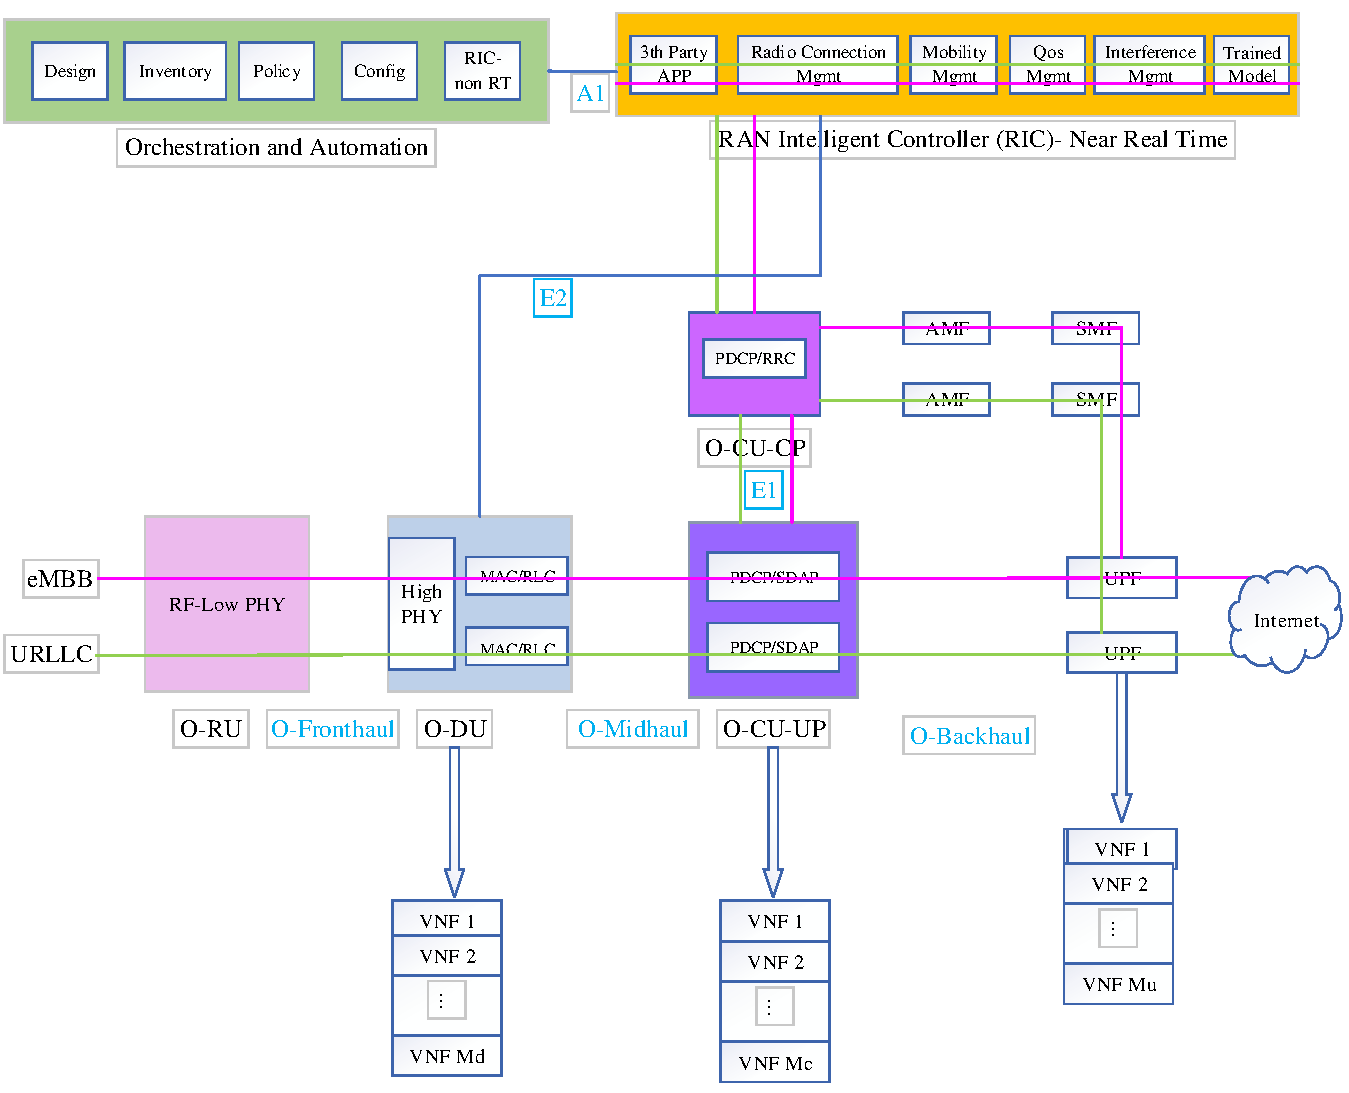
\includegraphics[scale = 0.4]{draw1.pdf}
  \caption{Network sliced ORAN system}
  \label{fig:c11}
\end{figure}

In this paper, as  depicted in Figure \ref{fig:c11}, the downlink of the ORAN system is studied.
\section{System Model and Problem Formulation}\label{systemmodel}

In this section, first, we  present the system model. Then, we obtain achievable data rates and delays for the downlink (DL) of the ORAN system. Afterward, we discuss about assignment of physical data center resources.
Finally, the main problem is expressed.
\subsection{System Model}
Suppose we have two service types includes eMBB and URLLC. Assume we have $S_1$ and $S_2$ different applications for the first and second service type, respectively ($S = S_1 + S_2$).
Assume we have $S$ preallocated slices serving these $S$ services; There are $S_1$ slices for the first service type (eMBB) and $S_2$ slices for the second service type (URLLC).
Each Service $s_j\in \{1,2,...,S_j \} $ consists of $U_{s_j}$ request from the 
single-antenna UEs which require certain QoS to be able to use the requested program($j \in \{1,2\}$ indicate service type).
There are different application request which fall into one of these service categories. Each application request requires specific QoS. Based on the request for the application and QoS, UE may be admitted and allocated to the resources.
Each slice $s_j \in \{1,2,...,S_j \}$, $j \in \{1,2\}$ consists of $K_{s_j}$, $j \in \{1,2\}$ preallocated virtual resource blocks that are mapped to Physical Resource Blocks (PRBs), $M_s^{d}$ VNFs for the processing of O-DU,  $M_s^{c}$ VNFs for the processing of O-CU-UP and $M_s^{u}$ VNFs for the processing of UPF.

Also, each VNF instance is running on the virtual machine (VM) that are using resources from the data centers. Each VM, requires enough resources of CPU, memory, storage and network bandwidth.

In addition, there are $R$ multi-antenna RU that are shared between slices. Each RU $r \in \{1,2,...,R \}$
has $J$ antenna for transmitting and receiving data. Moreover, all RUs, have access to PRBs.
\subsection{The Achievable Rate}
The SNR of $i^{th}$ UE requesting served at slice $s$ on PRB $k$ is obtained from
\begin{equation}\label{eq2}
\rho_{r,u(s,i)}^{k} =  \frac{|p_{r,u(s,i)}^{k}{\bold{h}_{r,u(s,i)}^{H \: k}} \bold{w}_{r,u(s,i)}^{k} g_{u(s,i)}^r|^2}{BN_0 + I_{r,u(s,i)}^{k}},
\end{equation} 
where $p_{r,u(s,i)}^{k}$ represents the transmission power from o-RU $r$ to $i^{th}$ UE served at slice $s$ on PRB $k$. 
${\bold{h}_{r,u(s,i)}^{k}} \in \mathbb{C}^{J}$ is the vector of channel gain of a wireless link from 
$r^{th}$ RU to the $i^{th}$ UE in $s^{th}$ slice. In addition, $\bold{w}_{r,u(s,i)}^{k} \in \mathbb{C}^{J}$ depicts the  transmit beamforming vector from $r^{th}$ RU to the $i^{th}$ UE in $s^{th}$ slice that is the zero forcing beamforming vector to minimize the interference which is indicated as below
\begin{equation}
\bold{w}_{r,u(s,i)}^{k} = {\bold{h}_{r,u(s,i)}^{k}}({\bold{h}_{r,u(s,i)}^{H \: k}} {\bold{h}_{r,u(s,i)}^{k}})^{-1}
\end{equation}
Moreover, $g_{u(s,i)}^r \in \{0,1\}$ is a binary variable that illustrates whether RU $r$ is mapped to the $i^{th}$ UE allocate to $s^{th}$ slice or not. 
Also, $BN_0$ denotes the power of Gaussian additive noise, and $I_{r,u(s,i)}^{k}$ is the power of interfering signals represented as follow
\begin{equation}
\begin{split}
I_{r,u(s,i)}^{k} &=
 \underbrace{\sum_{\substack{l=1 \\ l\neq i}}^{{U}_{s}} \gamma_{1}  p_{u(s,i)}^{k}\sum_{\substack{r'=1 \\ r'\neq r}}^{R}|{\bold{h}_{r',u(s,i)}^{H \: k}} \bold{w}_{r',u(s,i)}^{k} g_{u(s,i)}^{r'}|^2}_{\text{(intra-slice interference)}}\\
&+ \underbrace{\sum_{\substack{n = 1 \\ n\neq s}}^{S}\sum_{l=1}^{{U}_s} \gamma_{2}  p_{u(n,l)}^{k}\sum_{\substack{r'=1 \\ r'\neq r}}^{R}|{\bold{h}_{r',u(s,i)}^{H \: k}} \bold{w}_{r',u(n,l)}^{k} g_{u(n,l)}^{r'}|^2}_{\text{(inter-slice interference)}}\\
\end{split}
\end{equation}
where $\gamma_{1} = e^{k}_{r,u(s,i)}e^{k}_{r',u(s,l)}a_{u(s,i)}a_{u(s,l)}$
and $\gamma_{2} = e^{k}_{r,u(s,i)}e^{k}_{r',u(n,l)}a_{u(s,i)}a_{u(y,l)}$.
Where $a_{u(s,i)} \in \{0,1\}$ is a binary variable to depict user admission.
$e^{k}_{r,u(s,i)}$ is the binary variable to show whether the $k^{th}$ PRB is allocated to the UE $i$ in slice $s$, assigned to $r^{th}$ o-RU.

The achievable data rate for the $i^{th}$ UE request in the $s_{1}^{th}$ application of service type 1 (eMBB) can be written as $\mathcal{R}_{u(s_1,i)}^{e}$.
\begin{equation}\label{eq1}
\begin{split}
\mathcal{R}_{u(s_1,i)}^{e,r} &= \sum_{k=1}^{K_{s_1}} B \log_2({1+ \rho_{r,u(s_1,i)}^{k}})a_{u(s_1,i)} e^k_{r,u(s_1,i)},\\
\mathcal{R}_{u(s_1,i)}^{e} &= \sum_{r=1}^{R}\mathcal{R}_{u(s_1,i)}^{e,r} 
\end{split}
\end{equation}
where $B$ is the bandwidth of system. 
$\mathcal{R}_{u(s_1,i)}^{e,r}$ is the achievable rate of each RU $r$ to UE $i$ in slice $s_1$.
Since the blocklength in URLLC is finite, the achievable data rate for the $i^{th}$ UE request in the $s_{2}^{th}$ application of service type 2 (URLLC) is not achieved from Shannon Capacity formula. So, for the short packet transmission the achievable data rate is approximated from follow
\begin{equation}\label{eq11}
\begin{split}
\mathcal{R}_{u(s_2,i)}^{u,r} &= \sum_{k=1}^{K_{s_2}} B (\log_2({1+ \rho_{u(s_2,i)}^{k}})- \zeta_{u(s_2,i)}^{k}){\beta}_{u(s_2,i)}^{k}\\
\mathcal{R}_{u(s_1,i)}^{e} &= \sum_{r=1}^{R}\mathcal{R}_{u(s_2,i)}^{e,r} 
\end{split}
\end{equation}
Where ${\beta}_{u(s_2,i)}^{k}=a_{u(s_2,i)} e^{k}_{u(s_2,i)}$
and $\zeta_{u(s_2,i)}^{k} = log_2({e})Q^{-1}(\epsilon) \sqrt{\frac{C_{u(s_2,i)}^{k}}{N_{u(s_2,i)}^{k}}})$
Where, $\epsilon $ is the transmission probability, $Q^{-1}$ is the inverse of Q- function (Gaussian),
$C_{u(s_2,i)}^{k} = 1 - \frac{1}{(1+\rho_{u(s_2,i)}^{k})}$ depicts the channel dispersion of UE  $i$ at slice $s_2$, experiencing PRB $k$ and
$N_{u(s_2,i)}^{k}$ represents the blocklength of it. 
$\mathcal{R}_{u(s_1,i)}^{e,r}$ is the achievable rate of each RU $r$ to UE $i$ in slice $s_2$.
\subsection{Mean Delay}
In this part, the end to end mean delay for a service is obtained.
Suppose the mean total delay is depicted as $T_{tot}$.
\begin{equation}
\begin{split}
T_{tot} &=  T_{process} + T_{transmission} + T_{propagation}\\
T_{process} &=  T_{RU} + T_{DU} + T_{CU} + T_{UPF}\\
T_{transmission} &= T_{front} + T_{mid} + T_{back} + T_{trans2net} \\
T_{propagation} &= T_{front} + T_{mid} + T_{back} + T_{trans2net} \\
\end{split}
\end{equation}
%T_{tot} = T_{RU} + T_{front} + T_{DU} + T_{mid} + T_{CU} + T_{back} + T_{core} + T_{trans2net}
Total delay is sum of processing delay, transmission delay and propagation delay. 
The propagation delay is the time takes for a signal to reach to its destination. So it has a constant value based on the length of fiber link ($T = L/c$, where $L$ is the length of link and c is the speed of signal).
Here we assume the value of propagation delay is negligible compared to the rest.
\subsubsection{Processing Delay}
Assume the packet arrival of UEs follows a Poisson process with arrival rate $\lambda_{u(s,i)}$ for the $i^{th}$ UE of the $s^{th}$ slice.
Therefore, the mean arrival data rate of the $s^{th}$ slice in the UPF layer is $\alpha_{s}^1 = \sum_{u=1}^{U_s}a_{u(s,i)}\lambda_{u(s,i)}$, where $a_{u(s,i)}$ is a binary variable which indicates whether the $i^{th}$ UE requested $s^{th}$ service is admitted or not.

Assume the mean arrival data rate of the UPF layer for slice $s$ ($\alpha_{s}^U$) is approximately equal to the mean arrival data rate of the O-CU-UP layer ($\alpha_{s}^C$) and O-DU ($\alpha_{s}^D$). so $\alpha_{s} =\alpha_{s}^U \approx \alpha_{s}^C \approx \alpha_{s}^D$. since, by using Burke’s Theorem, the mean arrival data rate of the second and third layer which are processed in the first layer is still Poisson with rate $\alpha_{s}$.
It is assumed that there are load balancers in each layer for each service to divide the incoming traffic to VNFs equally. %\cite{frdl,luong2018novel,luong2018novel1}.
Suppose the baseband processing of each VNF is depicted as M/M/1 processing queue.
Each packet is processed by one of the VNFs of a slice. So, the mean delay for the $s^{th}$ slice in the first and the second layer, modeled as M/M/1 queue, is formulated as follow, respectively
\begin{equation}
\begin{split}
T_{DU}^{s} &= \frac{1}{\mu_d - \alpha_{s}/{M_s^{d}}},\\
T_{CU}^{s} &= \frac{1}{\mu_c - \alpha_{s}/{M_s^{c}}}\\
T_{UPF}^{s} &= \frac{1}{\mu_u - \alpha_{s}/{M_s^{u}}}\\
\end{split}
\end{equation}
Where $M_s^{d}$, $M_s^{c}$ and 
$M_s{u}$ are the variables that depict the sum of VNFs in O-DU, O-CU-UP and UPF, respectively. 
Moreover, $1/\mu_d$, $1/\mu_c$ and $1/\mu_u$ are the mean service time of the O-DU, O-CU and the UPF layers respectively.
Besides, $\alpha_{s}$ is the  arrival rate which is divided
by load balancer before arriving to the VNFs. The arrival rate of each VNF in each layer for each slice 
$s$ is $\alpha_{s}/{M_s^{i}}$ $ i \in \{d,c, u\}$.

In addition, $T_{RU}^{s}$ is the mean transmission delay of $s^{th}$ slice on the wireless link. The arrival data rate of wireless link is equal to the arrival data rate of load balancers for each service.
 %\cite{frdl}.
Moreover, it is assumed that the service time of transmission queue for each slice $s$ has
 an exponential distribution with mean $1/(R_{{tot}_s})$ and can be modeled as a M/M/1 queue.
 %\cite{frdl,luong2018novel,luong2018novel1,guo2016exploiting}. 
 Therefore,
the mean delay of the transmission layer is
\begin{equation}
 T_{RU}^{s} = \frac{1}{R_{{tot}_s} - \alpha_{s}};
\end{equation}
where, $R_{{tot}_s} = \sum_{u=1}^{U_s}a_{u(s,i)}R_{u(s,i)}$ is the total achievable rate of each service.
So the mean processing delay for each UE in slice $s$ is 
\begin{equation}
T_{process}^{s} =  T_{RU}^{s} + T_{DU}^{s} + T_{CU}^{s} + T_{UPF}^{s}
\end{equation}
\subsubsection{Transmission Delay}
The transmission delay is the amount of time required to push all the packets into the fiber link. 
Here, we have transmission delay in fronthaul, midhaul, backhaul and the link to transmit data to internet.
\begin{equation}
\begin{split}
T_{front} =& \frac{\alpha_{s}^{f}}{R_f} \\
T_{mid} =&  \frac{\alpha_{s}^{m}}{R_m} \\
T_{back} =& \frac{\alpha_{s}^{b}}{R_b} \\
T_{trans2net} =& \frac{\alpha_{s}^{t}}{R_t} \\
\end{split}
\end{equation}
Where, $R_f$, $R_m$, $R_b$ and $R_t$ are the rate of transmission in fronthaul, midhaul, backhaul and the link to transmit data to internet, respectively.
Furthermore, the mean arrival data rate of the each link ($\alpha_{s}^i$ , $i \in \{f,m,b,t\}$) is approximately equal to others ($\alpha_{s} \approx \alpha_{s}^i$ , $i \in \{f,m,b,t\}$).  
\subsection{Delay for URLLC}
As we know, UEs request URLLC services, require services with low latency.
For the M/M/1 system, the probability of the delay for each application $s$ in the UPF, CU, DU and RU is as follow, respectively
\begin{equation}
\begin{split}
P_r\{T_{UPF}^{s} \geq T_{UPF}^{max}\} &= e^{-(\mu_u - \alpha_{s}/{M_s^{u}})T_{UPF}^{max}}\\
P_r\{T_{CU}^{s} \geq T_{CU}^{max}\} &= e^{-(\mu_c - \alpha_{s}/{M_s^{c}})T_{CU}^{max}}\\
P_r\{T_{DU}^{s} \geq T_{DU}^{max}\} &= e^{-(\mu_d - \alpha_{s}/{M_s^{d}})T_{DU}^{max}}\\
P_r\{T_{RU}^{s} \geq T_{RU}^{max}\} &= e^{-(R_{{tot}_s} - \alpha_{s})T_{RU}^{max}}\\
\end{split}
\end{equation} 
So the probability of coincidence of these events is as follow
\begin{equation}
P_r\{E_1, E_2, E_3, E_4\} = A_1 A_2 A_3 A_4,
\end{equation}
Where $E_1 = T_{UPF}^{s} \geq T_{UPF}^{max}$, $E_2 =T_{CU}^{s} \geq T_{CU}^{max} $, $E_3 =T_{DU}^{s} \geq T_{DU}^{max} $ and $E_4 =T_{RU}^{s} \geq T_{RU}^{max} $.
Also $A_1=e^{-(\mu_u - \alpha_{s}/{M_s^{u}})T_{UPF}^{max}}$, $A_2=e^{-(\mu_c - \alpha_{s}/{M_s^{c}})T_{CU}^{max}}$, $A_3= e^{-(\mu_d - \alpha_{s}/{M_s^{d}})T_{DU}^{max}}$ and $A_4 = e^{-(R_{{tot}_s} - \alpha_{s})T_{RU}^{max}}$.
\subsection{Physical Data Center Resource}
Each VNF requires
physical resources that contain memory, storage, CPU and Network Bandwidth.
Let the required resources for VNF $f$ in slice $s$ is represented by a tuple as
\begin{equation}
\bar{\Omega}_{s}^f = \{\Omega_{M,{s}}^f, \Omega_{S,{s}}^f, \Omega_{C,{s}}^f, \Omega_{N,{s}}^f \},
\end{equation}
where $\bar{\Omega}_{s}^f\in \mathbb{C}^{4}$ and $\Omega_{M,{s}}^f, \Omega_{S,{s}}^f, \Omega_{C,{s}}^f, \Omega_{N,{s}}^f$ indicate the amount of required memory, storage, CPU and and Network Bandwidth, respectively.
Moreover, the total amount of required memory, storage, CPU and Network Bandwidth of all VNFs of a slice in DU, CU and UPF is defined as below, respectively
\begin{equation}
\begin{split}
&\bar{\Omega}_{\mathfrak{z},s}^{tot,d} = \sum_{f=1}^{M_{s}^d}\bar{\Omega}_{\mathfrak{z},s}^{f,d} \;\; \mathfrak{z} \in \{M, S, C, N\}.\\
&\bar{\Omega}_{\mathfrak{z},s}^{tot,c} = \sum_{f=1}^{M_{s}^c}\bar{\Omega}_{\mathfrak{z},s}^{f,c} \;\; \mathfrak{z} \in \{M, S, C, N\}.\\
&\bar{\Omega}_{\mathfrak{z},s}^{tot,u} = \sum_{f=1}^{M_{s}^u}\bar{\Omega}_{\mathfrak{z},s}^{f,u} \;\; \mathfrak{z} \in \{M, S, C, N\}.\\
\end{split}
\end{equation}
Where, $\bar{\Omega}_{\mathfrak{z},s}^{f,d}$, $\bar{\Omega}_{\mathfrak{z},s}^{f,c}$ and $\bar{\Omega}_{\mathfrak{z},s}^{f,u}$ are the amount of resource that a VNF required in DU, CU and UPF, respectively.
\begin{equation}
 \bar{\Omega}_{\mathfrak{z},s}^{tot} = \bar{\Omega}_{\mathfrak{z},s}^{tot,d}+ \bar{\Omega}_{\mathfrak{z},s}^{tot,c}+\bar{\Omega}_{\mathfrak{z},s}^{tot,u}
\end{equation} 
Also, there are $D_c$ data centers (DC), serving the VNFs. Each DC contains several servers that supply VNF requirements.
The amount of memory, storage, CPU and and Network Bandwidth is denoted by $\tau_{M_{j}}, \tau_{S_{j}}$, $\tau_{C_{j}} $ and $\tau_{N_{j}} $ for the $j^{th}$ DC, respectively
\begin{equation*}
\tau_j = \{\tau_{M_{j}}, \tau_{S_{j}}, \tau_{C_{j}}, \tau_{N_{j}} \},
\end{equation*}
In this system model, the assignment of physical DC resources to VNFs is considered. Let $y_{s,d}$ be a binary variable indicating whether the $d^{th}$ DC is allocated the resources to the VNFs of $s^{th}$ slice or not.
\subsection{Problem Statement}
%In this system, the goal is to minimize the cost of the system.
Power of each O-RU is obtained as below
\begin{equation}
P_r =  \sum_{s=1}^{S} \sum_{i=1}^{U_v} \sum_{k=1}^{K_s}p_{r,u(s,i)}^{k}a_{u(s,i)} e^{k}_{r,u(s,i)}g_{u(s,i)}^r.
\end{equation}
%The total power cost of O-RUs for transmitting data to UE is depicted as follow
%\begin{equation}
%P_{tot} = \sum_{r=1}^{R}P_r
%\end{equation}
Assume the power consumption of baseband processing at each DC $d$ that is connected to VNFs of a slice $s$ is depicted as
$\phi_{s}$. So the total power of the system for all active DCs that are connected to slices can be represented as
\begin{equation*}
\textstyle \phi_{tot} = \sum_{s=1}^{S}\phi_{s} + \sum_{d=1}^{D_c}z_d \psi_d .
\end{equation*}
Where,$z_d$ is shown that whether the $d^{th}$ DC is turned on or not and $\psi_d$ is a static cost when a DC is active.
\begin{equation}
  z_d =
    \begin{cases}
      1 & \sum_{s=1}^{S}y_{s,d} \geq 1 \\
      0 & \text{otherwise}
    \end{cases}       
\end{equation}  
In addition, $\phi_{s}$ is obtained from below
\begin{equation}
\phi_{s} = M_s^u \phi_s^u + M_s^c \phi_s^c+ M_s^d \phi_s^d
\end{equation}
Where, $\phi_s^u$, $\phi_s^c$ and $\phi_s^d$ are the static cost of energy in UPF, CU and DU, respectively. 
So the optimization problem is formulated as follow.
The aim of this paper is to maximize the sum rate of all UEs  with the presence of constraints which is written as follow,
\begin{subequations}
\begin{alignat}{4}
\max\limits_{\boldsymbol{P}, \boldsymbol{A}, \boldsymbol{E}, \boldsymbol{M}, \boldsymbol{G}, \boldsymbol{Y} }   \quad &  \sum_{s=1}^{S}\sum_{i=1}^{U_s}R_{u_{(s,k)}} \ \\
\text{subject to} \quad  &  P_r \leq P_{max} \quad \forall r
 \label{c11} \\
&p_{r,u(s,i)}^{k}  \geq 0  \quad \forall i,\forall r,\forall s, \forall k,\label{c12} \\
&\mathcal{R}_{u_{(s_1,i)}}^e \geq  a_{u(s_1,i)}\mathcal{R}_{min}^{s_1,e} \quad \forall s_1, \label{c13} \\
&\mathcal{R}_{u_{(s_2,i)}}^u \geq  a_{u(s_2,i)}\mathcal{R}_{min}^{s_2,u} \quad \forall s_2, \label{c14} \\
& \sum_{s=1}^{S}\sum_{i=1}^{U_s}R_{u_{(s,k)}}^r \leq C_{max}^r \quad \forall r, \label{c15}\\ 
&T_{tot}^s \leq T_{tot}^{max,s} \quad \forall s,\label{c16} \\
& P_r\{E_1, E_2, E_3, E_4\} \leq \epsilon_s \quad \forall s_2, \label{c166}\\
&a_{u(s,i)} \leq a_{u(s,i)}\sum_{r}g^r_{u(s,i)}  \quad \forall s,\forall i, \label{c17}  \\
& a_{u(s,i)}g^r_{u(s,i)} \leq a_{u(s,i)}g^r_{u(s,i)}\sum_{k =1}^{K_s} e^{k}_{r,u(s,i)}  \quad \forall s,i , \label{c18} \\
& \phi_{tot}  \leq \phi_{max}, \label{c19} \\
 &\textstyle \sum_{s=1}^{S} y_{s,d} \bar{\Omega}_{\mathfrak{z},s}^{tot}  \leq   \tau_{\mathfrak{z}_d} 
 \quad \forall d, \forall \mathfrak{z}\in \mathcal{E}; \label{c20}
\end{alignat}
\label{constraints}
\end{subequations}
where $\boldsymbol{P} =[p_{u(s,i)}] \:\: \forall s , \forall i $, is the matrix of power for UEs, $\boldsymbol{A} =[a_{u(s,i)}] \:\: \forall s , \forall i $ denotes the binary variable for UE admission,
$\boldsymbol{E} =[e_{r,u(s,i)}^k] \:\: \forall s , \forall i \forall r, \forall k$ indicate the binary variable for PRB association. Moreover, $\boldsymbol{G} =[g_{u(s,i)}^r] \:\: \forall s , \forall i \forall r$ is a binary variable for O-RU association. Furthermore, $M = [M_s^d, M_s^c, M_s^u] \:\: \forall s$ is the matrix that shown the number of VNFs in each layer of slice and $\boldsymbol{Y} =[y_{s,d}]  \:\: \forall s ,  \forall d $ is a binary variable shown whether
the physical DC is mapped to a VNFs of a slice or not.
Also, $\eta$ is weighted variable to value between the benefit and the cost term of objective function.
\eqref{c11}, and \eqref{c12}, indicate that the power of each RU do not exceed the maximum power, and the power of each UE is a positive integer value, respectively. 
Also \eqref{c13} and \eqref{c14} shows that the rate of each UE requesting eMBB and URLLC is more than a threshold, respectively.
\eqref{c15} and \eqref{c16} expressed the limited capacity of the fronthaul link, and the limited delay of receiving signal, respectively.
\eqref{c16} is a reliability condition that the delay in each layer should be less than threshold.
\eqref{c17} and \eqref{c18} guarantee that if a UE in admitted by the system, O-RU and PRB is associated to it, respectively.
In addition, \eqref{c19} indicate that the static cost of energy of VNFs in each slice do not exceed from the threshold. 
Moreover, in \eqref{c20}  $\mathcal{E} = \{M,S,C, N\}$ and the constraint supports
that we have enough physical resources for VNFs of each slice.


\bibliographystyle{IEEEtran}
\bibliography{ref}
\end{document} 